\documentclass[conference]{IEEEtran}
\IEEEoverridecommandlockouts
% The preceding line is only needed to identify funding in the first footnote. If that is unneeded, please comment it out.
\usepackage{cite}
\usepackage{amsmath,amssymb,amsfonts}
\usepackage{hyperref}
\usepackage{algorithmic}
\usepackage{graphicx}
\usepackage{booktabs}
\usepackage{textcomp}
\usepackage{xcolor}
\def\BibTeX{{\rm B\kern-.05em{\sc i\kern-.025em b}\kern-.08em
    T\kern-.1667em\lower.7ex\hbox{E}\kern-.125emX}}
\begin{document}


\title{Composition of concrete and its influence on compressive strength\\
%{\footnotesize \textsuperscript{*}Note: Sub-titles are not captured in Xplore and
%should not be used}
%\thanks{Identify applicable funding agency here. If none, delete this.}
}

\author{\IEEEauthorblockN{Filipe P. de Farias}
\IEEEauthorblockA{\textit{Department of Teleinformatics Engineering} \\
\textit{Federal University of Ceará}\\
Fortaleza, Brazil \\
filipepfarias@fisica.ufc.br}
\and
\IEEEauthorblockN{Yvo J. M. Sales}
\IEEEauthorblockA{\textit{Department of Teleinformatics Engineering} \\
\textit{Federal University of Ceará}\\
Fortaleza, Brazil \\
yvo@gtel.ufc.br}
}

\maketitle

\begin{abstract}
The compressive strength of concrete impacts directly on its application. The difference between the concrete for columns or beams and the concrete for pavements is mainly due the compressive strength it is able to resist. In this work, we perform unconditional and class-conditional monovariate and bivariate analysis as well as multivariate analysis (Principal Component Analysis) in the concrete database collected by UCI Machine Learning Repository (University of California, Irvine).
\end{abstract}

\begin{IEEEkeywords}
concrete, compresive, strength, machine, learning, pre-processing
\end{IEEEkeywords}

\section{Introduction}
The applications of the concrete depends directly on its compressive strength. This works tries to predict this compressive strength and to classify when the concrete is proper to be applied in structures. For instance the concrete for columns or beams needs to have more compressive strength than the one for pavement, in general. In the UCI database the concrete is tested with different components concentrations and different curing time (ages). 

\section{Data description}

The composition of each of the $N$ concrete samples is given by the concentrations (kg/m\textsuperscript{3}) of $D$ components: Cement, Blast Furnace Slag, Fly Ash, Water, Superplasticizer, Coarse Aggregate and Fine Aggregate. Each sample has its Age (day) and the measured Concrete compressive strength (MPa).

\begin{table}[htp]
\caption{Data Description}
\begin{center}
  \begin{tabular}{@{} clc @{}}
    \toprule
    Component & Description & Unit \\ 
    \midrule
    $D_1$ & Cement & kg/m\textsuperscript{3} \\ 
    $D_2$ & Blast Furnace Slag & kg/m\textsuperscript{3} \\ 
    $D_3$ & Fly Ash & kg/m\textsuperscript{3} \\ 
    $D_4$ & Water & kg/m\textsuperscript{3} \\ 
    $D_5$ & Superplasticizer & kg/m\textsuperscript{3} \\ 
    $D_6$ & Coarse Aggregate & kg/m\textsuperscript{3} \\ 
    $D_7$ & Fine Aggregate & kg/m\textsuperscript{3} \\ 
    $D_8$ & Age & days \\ 
	\midrule
    N & 1030 samples&  \\ 
    \bottomrule
  \end{tabular}
\end{center}
\label{Data Description}
\end{table}%

The concrete was stratified into $L=3$ classes\cite{b1}. This is, the concrete which is weak and not recommended for structures $L_1$, the \emph{Non-standard}. The concrete whose strength is in a range that can be applied to structures is classified as $L_2$, or \emph{Standard}. And the high performance concrete $L_3$, \emph{High-standard}.

The observations $Y$ are the measured compressive strengths of each sample and, as the predictors $D_1 - D_7$, are continuous. The Age ($D_8$) of the concrete is extremely discrete.

\section{Data Analysis}

In order to do future works, an analysis of the data is needed to understand them and perform their validation.

\subsection{Unconditional Mono-variate Analysis}

The statistics of each predictor is obtained performing a mono-variate analysis. At this step is possible to verify how the data is distributed.

\begin{table}[htp]
\caption{Data Statistics Summary}
  \centering
  \begin{tabular}{@{} crrr @{}}
    \toprule
     & Mean & STD & Skewness \\ 
    \midrule
    $D_1$ & 281.16 & 104.506 & 0.50873 \\ 
    $D_2$ & 73.89 & 86.279 & 0.79955 \\ 
    $D_3$ & 54.18 & 63.997 & 0.53657 \\ 
    $D_4$ & 181.56 & 21.354 & 0.07451 \\ 
    $D_5$ & 6.20 & 5.973 & 0.90588 \\ 
    $D_6$ & 972.91 & 77.754 & 0.04016 \\ 
    $D_7$ & 773.58 & 80.176 & 0.25264 \\ 
    $D_8$ & 45.66 & 63.169 & 3.26441 \\       
    \bottomrule
  \end{tabular}
\label{Data Statistics Summary}
\end{table}%

In Table~\ref{Data Statistics Summary} it is possible to see that the data are not \emph{highly skewed}, but yet are needed to be normalised to zero mean and standard unitary variation. This can be easier shown in Figure~\ref{}.

\begin{figure}[htbp]
\centerline{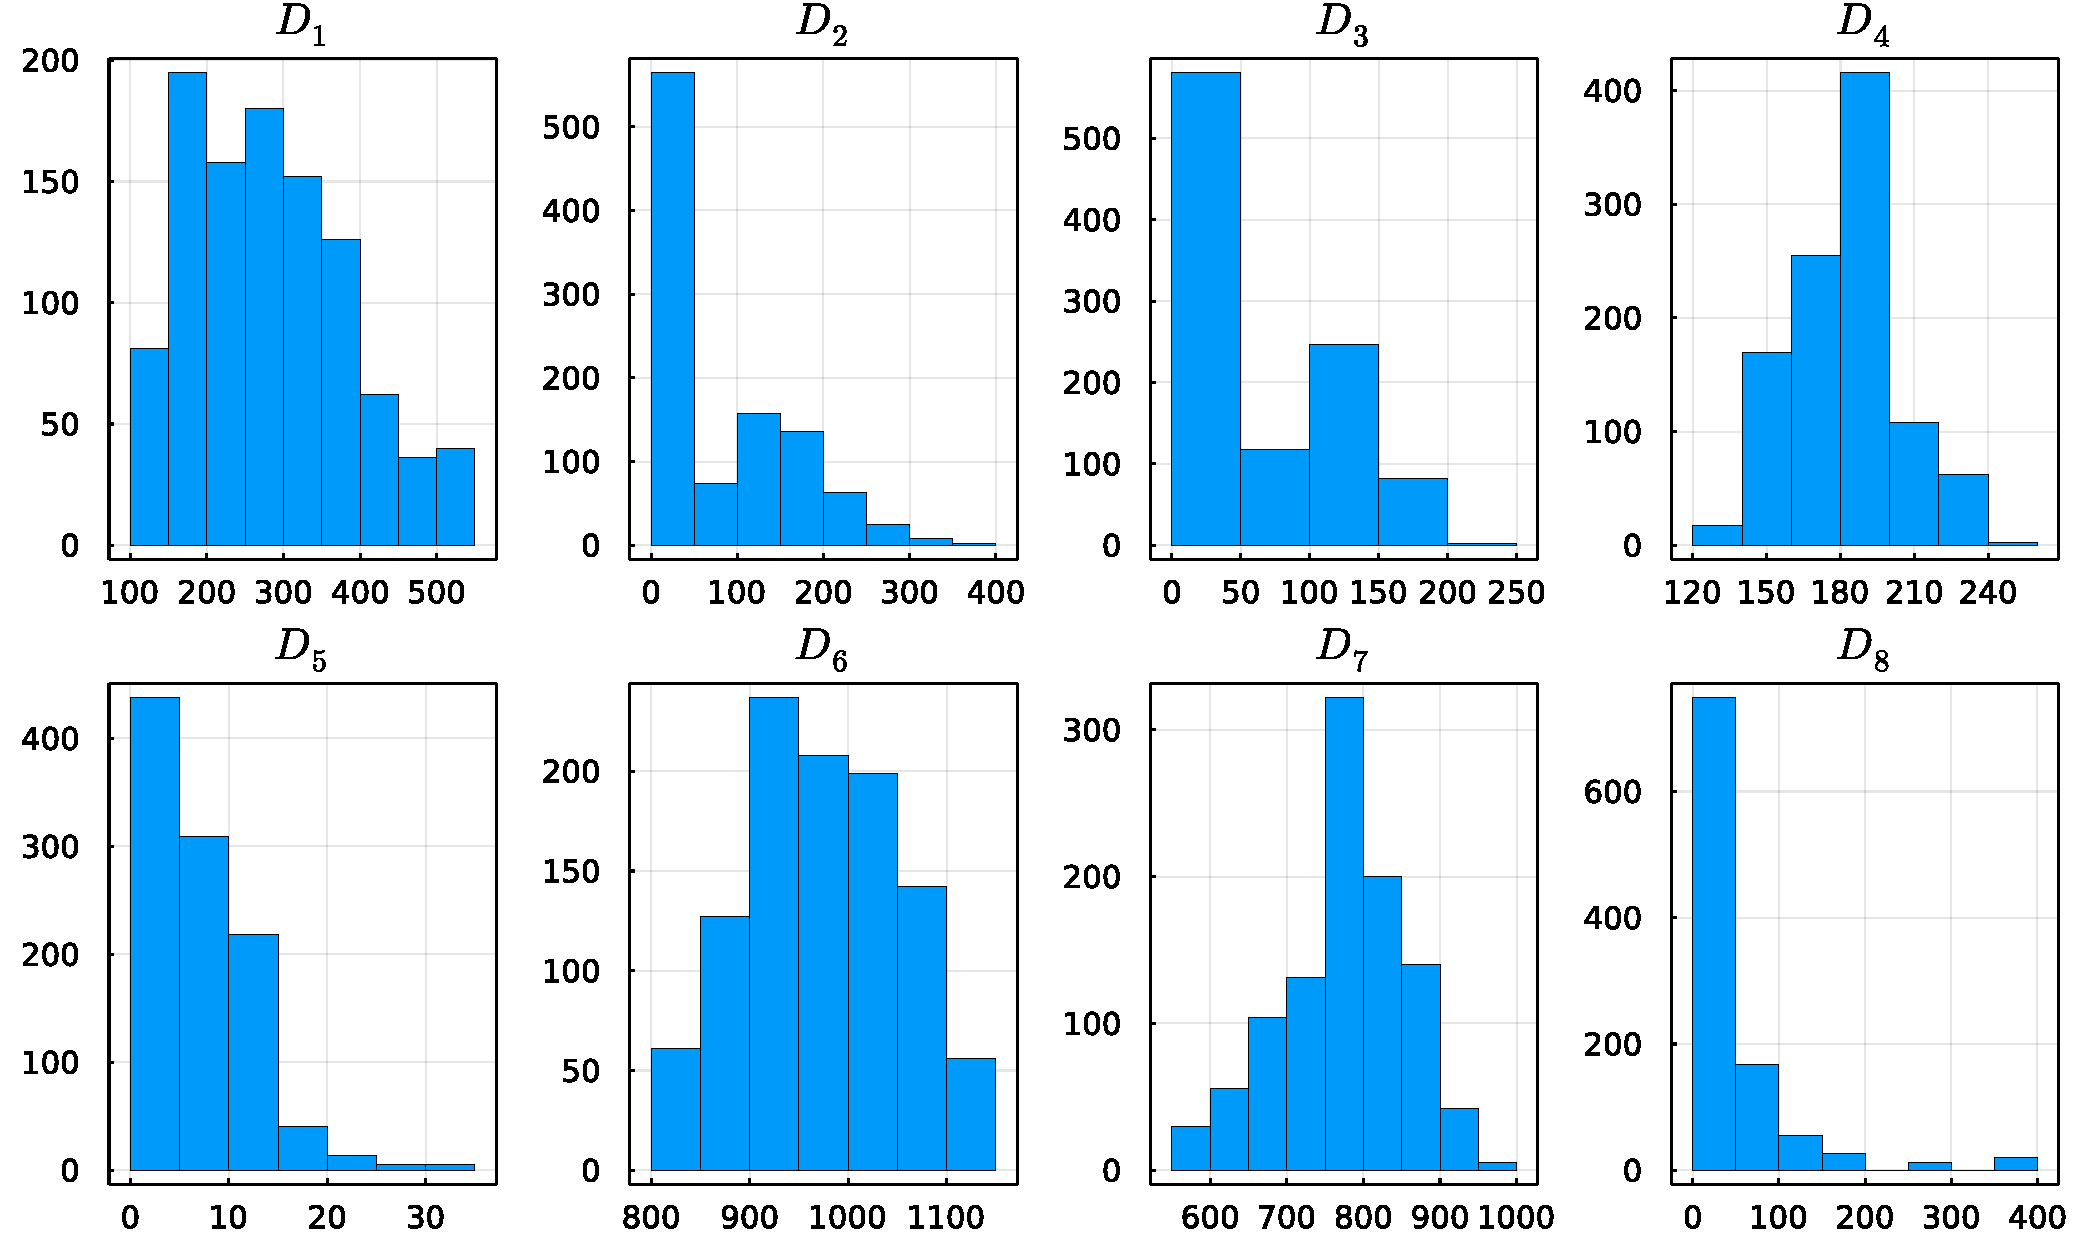
\includegraphics[width=\columnwidth]{../figures/monovariate_histograms_allcategories}}
\caption{Example of a figure caption.}
\label{fig}
\end{figure}

An interesting fact is that the components that, in general are not absent in the concrete composition has the lower skewness. These components are beyond Cement and Water, Coarse and Fine Aggregates. The other components have higher skewness due to the fact they are optional in concrete mixture, thus they allow to have zero values in some samples. Another seeable fact is the discreteness of the Age values. In general the concrete achiev
es the \emph{cure} at the end of 28 days. this explains the size of the bins between 0 and 100. The other cure periods are sampled in dataset to test its influence in compressive strenght.

\subsection{Class-conditional mono-variate analysis}

\begin{figure}[htbp]
\centerline{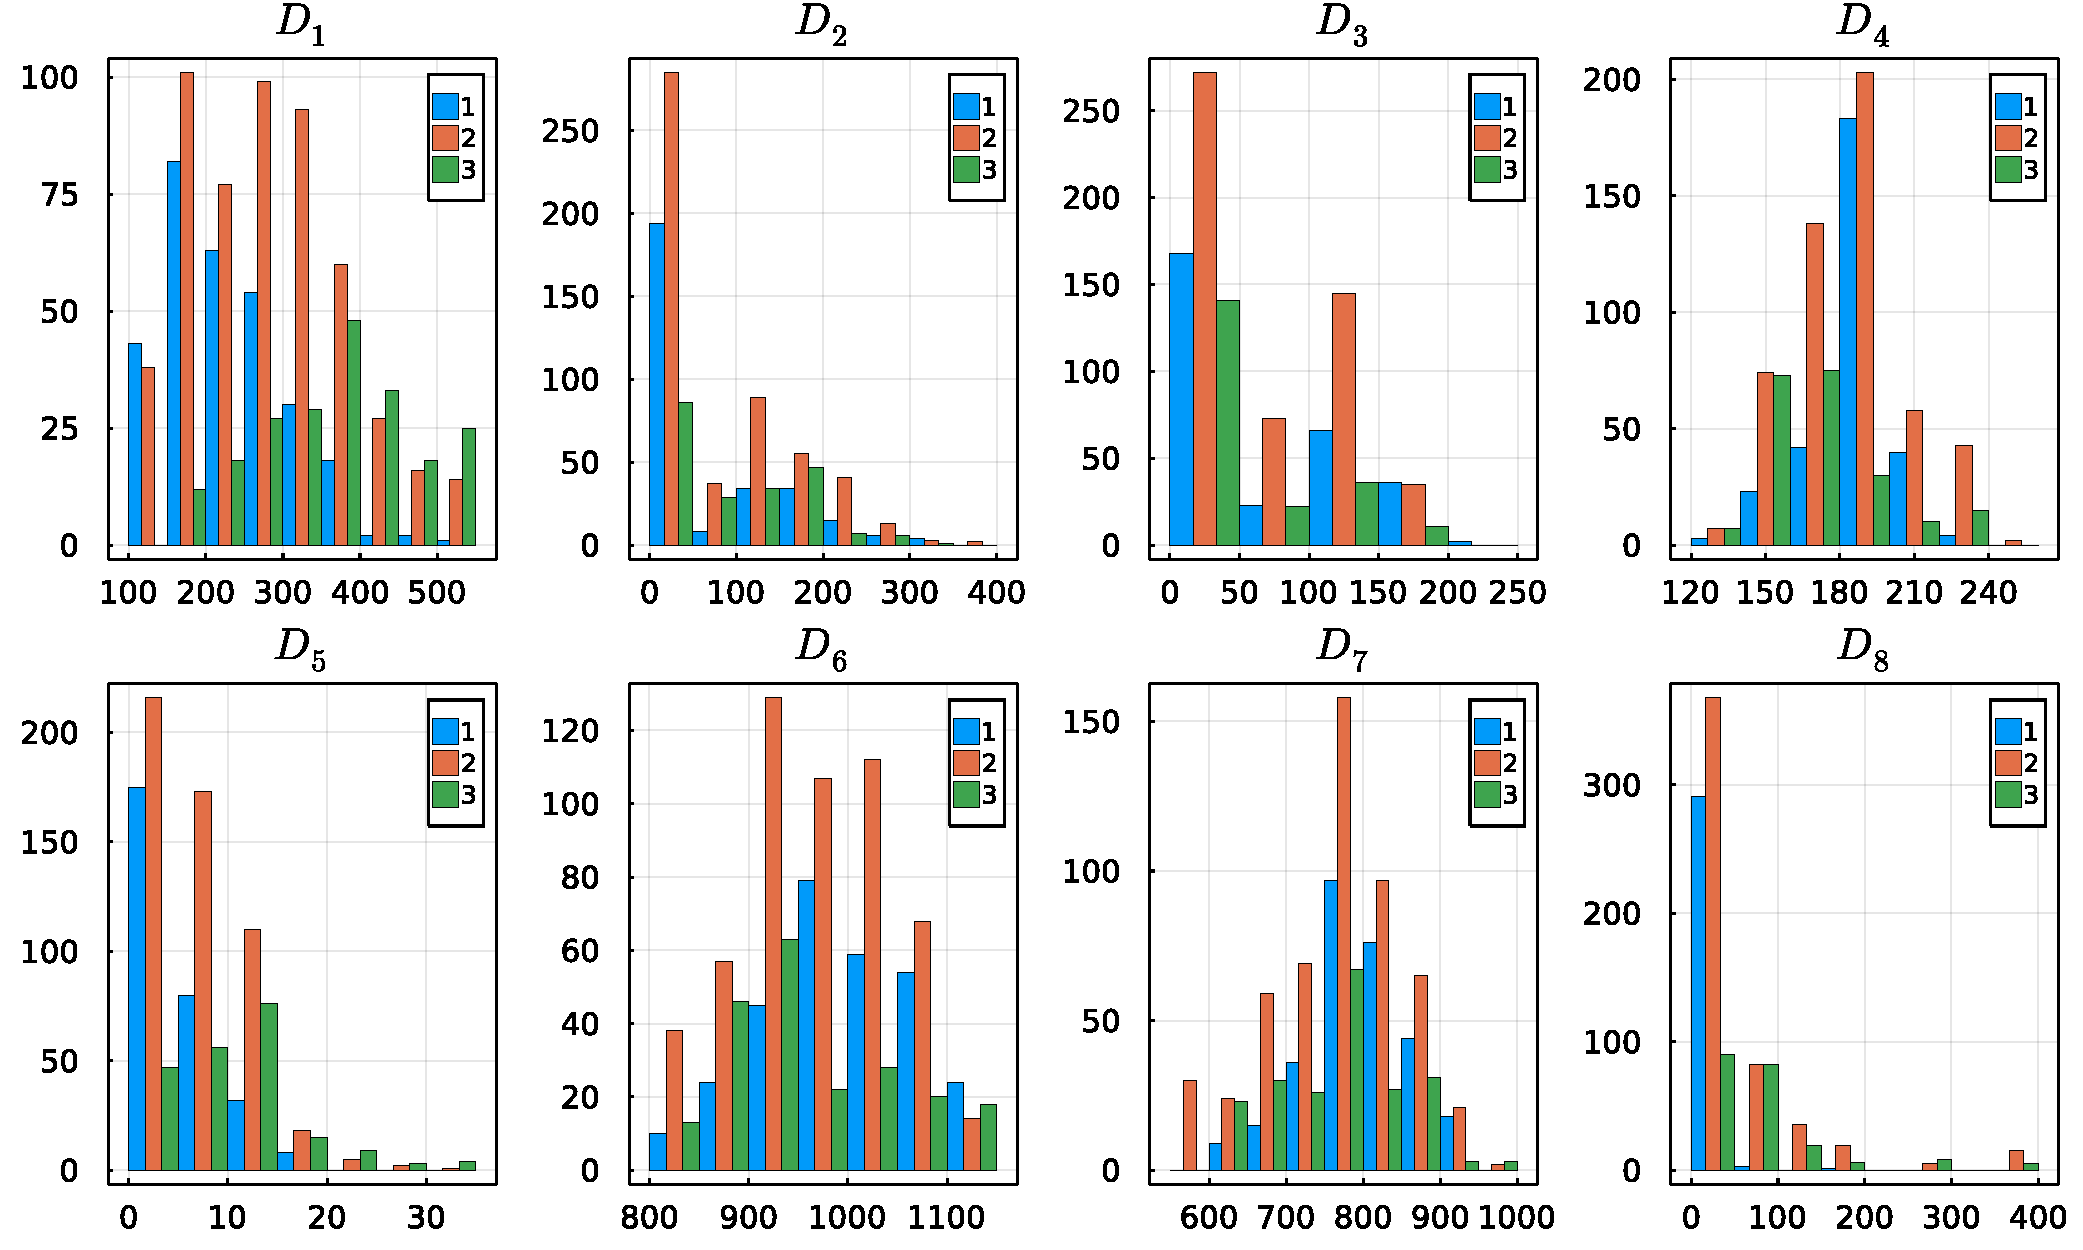
\includegraphics[width=\columnwidth]{../figures/monovariate_histograms_classcond}}
\caption{Example of a figure caption.}
\label{fig}
\end{figure}

As mentioned before, a Gaussian like distribution can distribution can be noticed on the components except the Superplasticizer and the Age. On the other ones, as in Fly Ash, there's a large number of zeros. This behaviour is repeated on the three classes. There's no apparent discretion between the classes too. In the trial to adjust the data of each component class into a Gaussian distribution, it was noticed that a mixture model would fits better given we have exact zeros and a distribution of non zero values. This is reasonable because the zero values are the representative absence of the component.

\subsection{Class-conditional bi-variate analysis}

In the pairwise comparison of the predictors, only in $(D_4,D_5)$, the Superplasticizer and Water concentrations, has a prominent negative correlation. The other predictors seemed do not have stronger correlations. Then it was not considered eliminate predictors to simplify the problem. In the same manner mentioned before, visually it was not possible to specify a predictor that might separate the classes.

The statistics of each predictor is at Table~[].

\begin{figure}[htbp]
\centerline{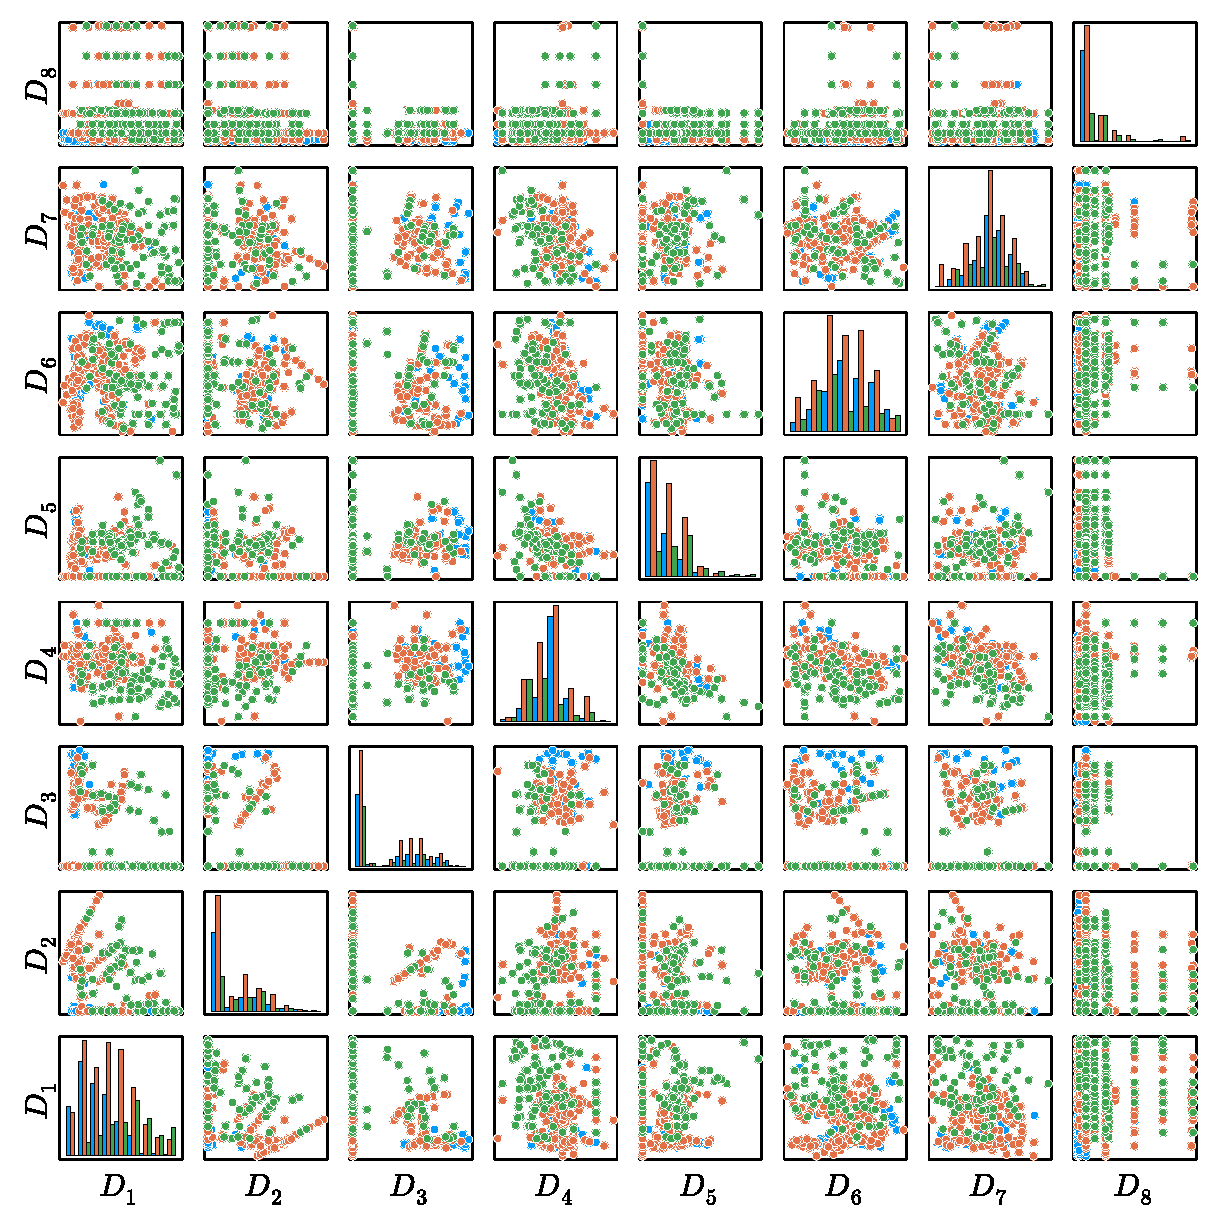
\includegraphics[width=\columnwidth]{../figures/bivariate_histograms_allclass}}
\caption{Example of a figure caption.}
%\label{fig}
\end{figure}

\begin{figure}[htbp]
\centerline{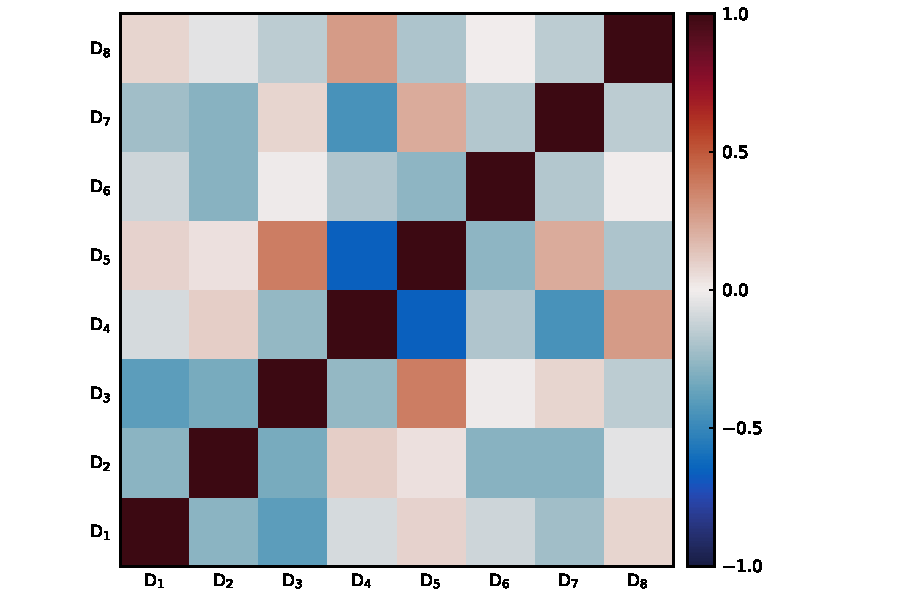
\includegraphics[width=\columnwidth]{../figures/predictors_corr_matrix.pdf}}
\caption{Example of a figure caption.}
\label{fig}
\end{figure}

\subsection{Unconditional multi-variate analysis (PCA)}

How the PCs comprises the original variance is plotted on Figure~[]. The original predictors are projected onto the PCs space, Figure~[]. Note the first component, the cement $D_1$ has less information in the first two PCs components. An interesting fact about this is to know that the cement can even turns the concrete weaker to compression as long its concentration grows. The compression strength will be given by the aggregate and some chemicals, which are the predictors of major norm in the projection.

In the Figure~[] is shown the projection of the original data onto de first two PCs. The classes are highly overlapping and another methods are needed to allow the classes to be separeted.

\begin{figure}[htbp]
\centerline{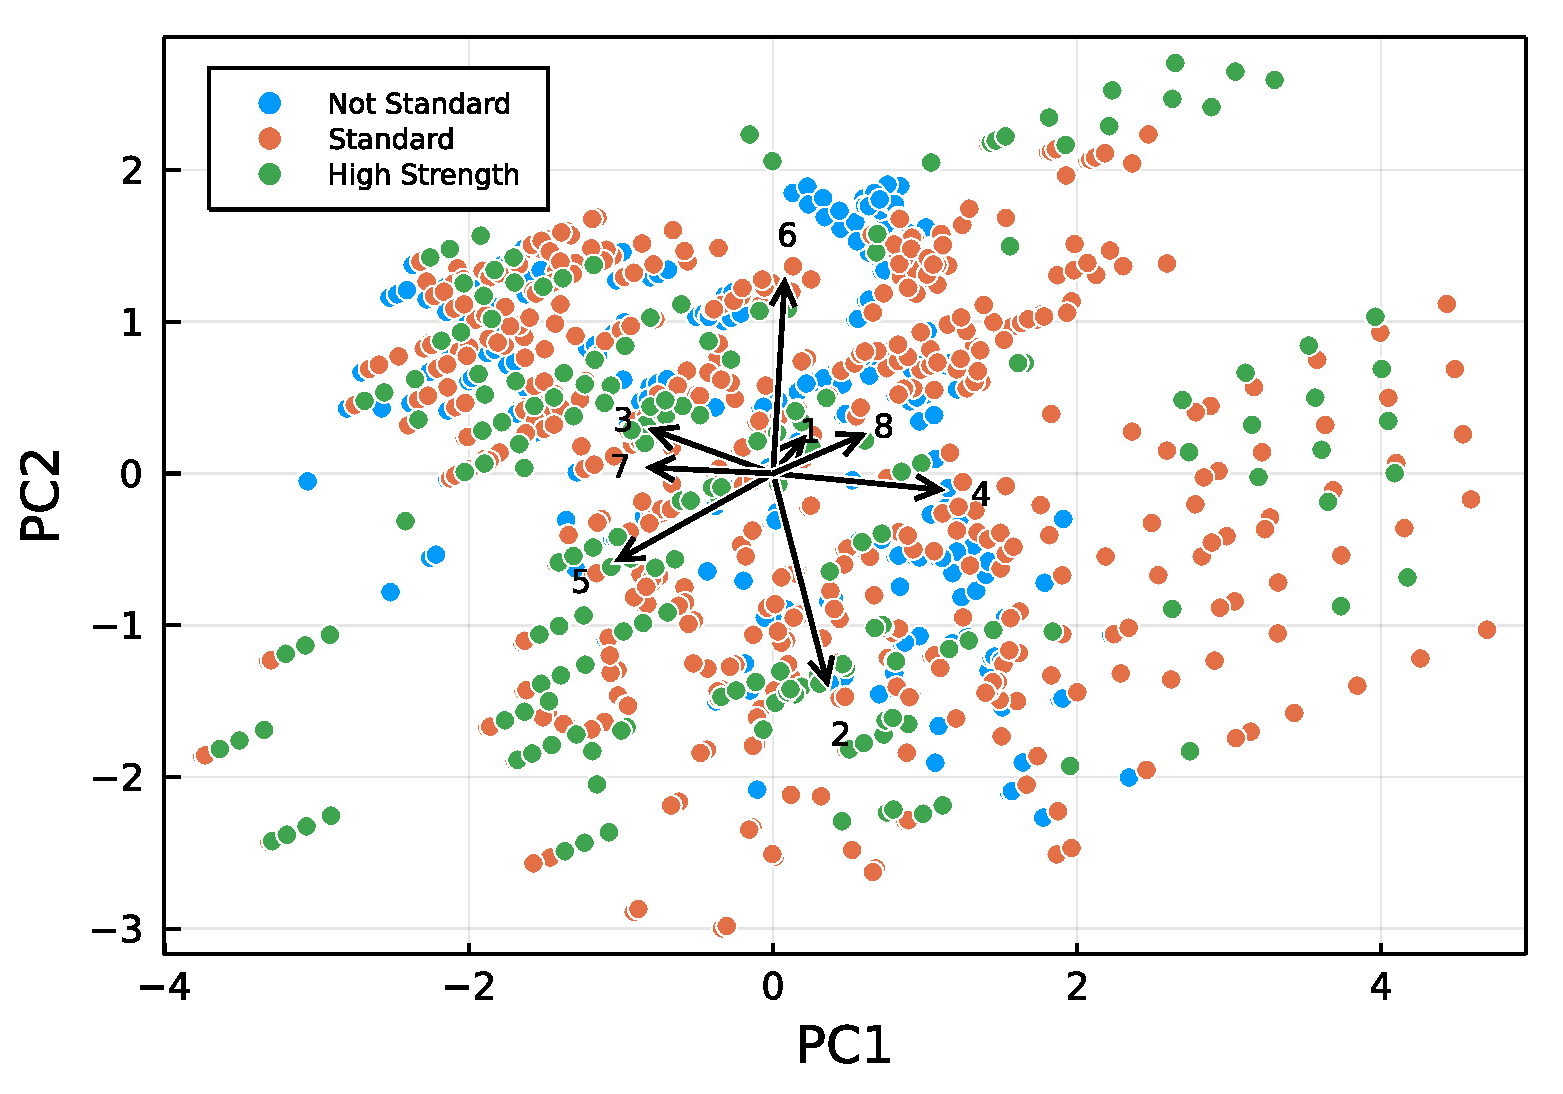
\includegraphics[width=\columnwidth]{../figures/pca_scatter_plot}}
\caption{Example of a figure caption.}
%\label{fig}
\end{figure}

\begin{figure}[htbp]
\centerline{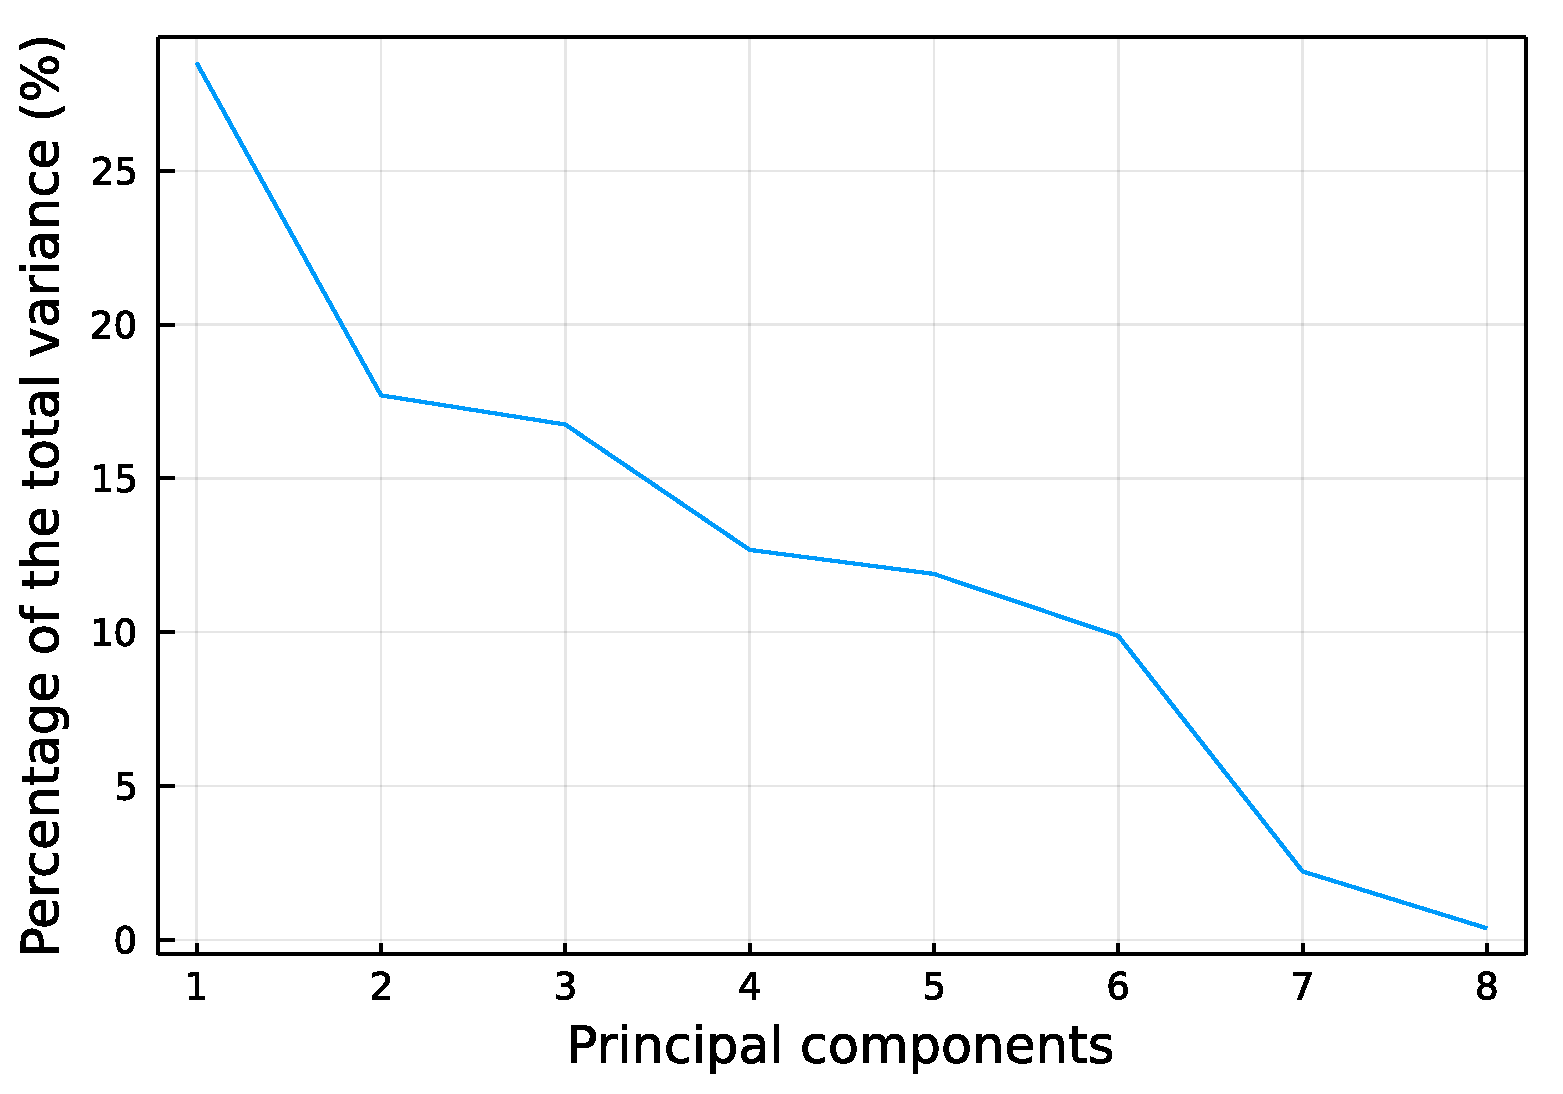
\includegraphics[width=\columnwidth]{../figures/pca_variance}}
\caption{Example of a figure caption.}
%\label{fig}
\end{figure}

\section{Conclusion}

The database of concrete is not easy to analyse if no knowledge about the problem of the mixture was studied. In none of the analysis the data have be shown as separable on the initially determined classes. The next step is to try to perform regression to model the compressive strength itself before trying to classify the samples.

\begin{thebibliography}{00}
\bibitem{b1} ``Different types of concrete grades and their uses'' \url{https://www.baseconcrete.co.uk/different-types-of-concrete-grades-and-their-uses/}. Accessed on 25/05/2021.
\bibitem{b2} Tibshirani, Robert, et al. The Elements of  Statistical Learning:  Data Mining, Inference, and Prediction. Alemanha, Springer New York, 2009.
\end{thebibliography}
\end{document}